\documentclass{www2010-submission}
\usepackage{algorithm}
\usepackage{algorithmic}
\begin{document}

\title{Leveraging Semantics for a Deep Web Question and Answering System} 
\numberofauthors{1}
\author{
	 \alignauthor Christan Grant, Clint P. George, Joseph N. Wilson, Peter J. Dobbins, Jeff T. Depree, Christopher A. Shields and Joir-dan Gumbs\\
	 \affaddr{Dept. of Computer Science, University of Florida} \\ \affaddr{ Gainesville, Florida, USA} \\
\email{cgrant@cise.ufl.edu, cpj@cise.ufl.edu, jnw@cise.ufl.edu, pjd@cise.ufl.edu, jdepree@cise.ufl.edu, cas@cise.ufl.edu, jg@cise.ufl.edu}
}

\date{April 26,2010}

\maketitle

\begin{abstract}
- It is difficult to answer question that change over time
- However, if the method of answering the question can be realized, the question can be easily answered
- We are building a system that supports a learning how to answer particular questions
- We can answer questions that are semantically similar to our store of questions
- We do this by building a semantic library ...
\end{abstract}

\category{H.4.m}{Information Systems Applications}{Miscellaneous}

\terms{SSQ}

\keywords{Questions Answering, re-finding}

\section{Introduction}
% Christan
- IEEE potentials article talks discussed the idea of using the beaten trail. To solve problems
- Typical search engines have several repeat queries.
- We believe that treating these repeat visits as special visits will enhance user search experience
- To demonstrate this concept we are building a tool that facilitates reuse in the specific domain of question answering
- 
- 

\section{Statistical Hierarchy}
\subsection*{Class Hierarchy}
%clint
\subsection*{Markov Blanket}
%joir-dan
Once the semantic hierarchy is created, the next step is to create training data for the system. The task is then to grab the pages, build a corpus relating to a given category, and then compile the information in a meaningful way. The overall goal is to grab enough information to properly characterize a category while limiting the amount of unnecessary content within the corpus. The problem with this approach is the page density varies greatly across the heterarchy. Each category within the DBpedia/ Wikipedia heterarchy contains a set of information pages, P, that correspond to concepts that share said category. Considering that the categorical structure is a directed acyclic graph (Suchanek et al., 2008), we consider the use of a Markov Blanket (Friedman et al., 1997) in describing a particular category. The category's that The assumption is that a node can be fully described by its ancestor, descendant, and spousal nodes (parent node of subcategory not equal to the category). While this does not completely solve the issue of a category residing in a sparse area of the graph, the amount of information that can be obtained per blanket is usually more helpful than per category.

Consider the abbreviated Markov blanket for the category Basketball:
%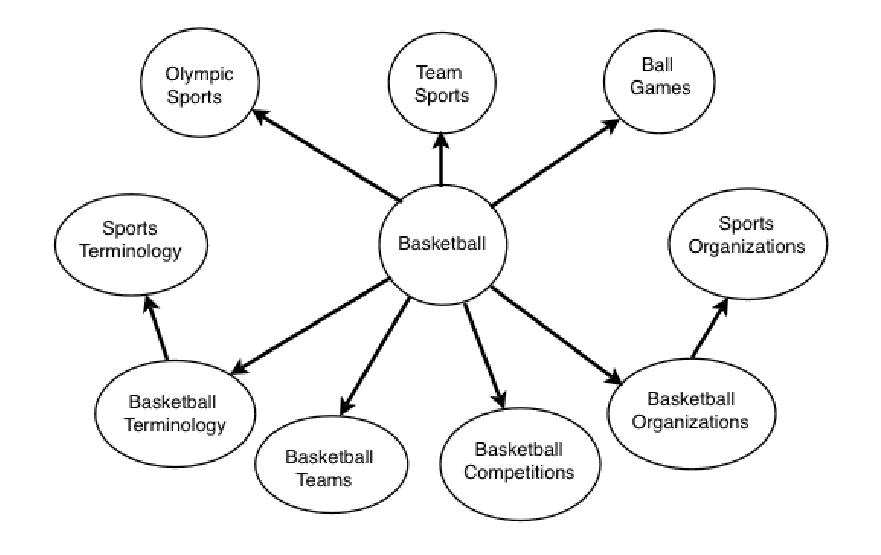
\includegraphics[width=1in,height=1in,viewport=0 0 100 100]{abbreviated_basketball_blanket.png}

The subcategories of the category Basketball (... Basketball Organizations, Basketball Competitions, Basketball Terminology, Basketball Teams...) can be seen as grabbing information specifc to the category. The supercategories (Ball Games, Olympic Sports, Team Sports) place the category in a higher perspective, abstractly describing basketball as a concept. The spousal categories are an abstract description of the subcategories.

Clustering the categories alone does not guarantee adequate corpus creation. Since the above model relies on the subcategories to describe specifcs of a given category, the ideal situation would be that the subcategories have many more pages than the supercategories and that there is a signifcant amount of information per page. In the case of Wikipedia, there are an average of 25.7 pages per category (Yu et al., 2007). The assumption for collecting the training data is the more subcategory data we have, the more detailed our description of our category. Considering that there are many categories that have much more than 26 pages, we instituted a PlusOne mechanism to extract extra information. This mechanism checks if a subcategory has an adequate number of pages a to fully describe its subtopic. We set this number to 10 * average, or 39. level represents how many extra levels we are to go down in the hierarchy, if necessary. SubjectSet is the overall set of all pages associated with the blanket structure along with any plusOne subjects obtained.

\begin{algorithm}
\caption{Blanket Subject Retrieval}
\label{alg1}
	\begin{algorithmic}
		\STATE BlanketSubjectRetrieval(blanket, maxLevel):
		\FOR{category c in blanket}
			\STATE subjectSet.add(grabSubjects(c))
			\STATE diff = afterSize - beforeSize
			\IF{ diff \leq \alpha and c is a subcategory}
				\STATE PlusOneMechanism(category, maxLevel)
			\ENDIF
		\ENDFOR
		\STATE return subjectSet
	\end{algorithmic}
\end{algorithm}



\begin{algorithm}
\caption{Plus One Mechanism}
\label{alg2}
	\begin{algorithmic}
		\STATE PlusOneMechanism(category, level)
		\STATE plusOneSet = grabPlusOneSubcategories(category)
		\FOR{ subcategory in plusOneSet}
			\STATE subjectSet.add(grabSubjects(subcategory))
			\STATE diff = afterSize - beforeSize
			\IF{ diff \leq \alpha \and level \gt 0}
				\STATE PlusOneMechanism(subcategory, level - 1);
			\ENDIF
		\ENDFOR
	\end{algorithmic}
\end{algorithm}


The overall mechanism does not take into account the amount of information within each page, but generally that can be ignored when considering the size of the blanket corpus when we extract the text from the Wikipedia subject pages. Using this method on the category Basketball, we can construct a corpus of 1843 subject pages and 1,301,006 terms.

When a category's corpus is built, we then build our n-gram frequency distributions and store them in a database for the NLP processing.



\section{Semantic Query Representation}
% Christan - fois

\section{Building Query Store}
\subsection{Query Resolution Recorder}
% Chris
\subsection{Generalization}
% Christan
The response pages created by querying web forms are
dynamically generated with a templated structure.
This
generalization per page is done using the GenPath algorithm developed by Badica et al. \cite{Badica06}. Additionally, the community may be able to answer a particular SSQ using many different page interactions. Therefore, we proposed a method of generalizing extraction path to a result across pages. This method removes unnecessary page interactions and finds the shortest path to the result pages.

The websites that are wrapped are highly susceptible to structural changes \cite{TanZMG07}. Generalizing the extraction paths help to overcome small structural changes. If a website changes to the point where a QRM is no longer useful, the QRM not considered fresh. Morpheus allows users to rate the freshness of QRMs.


\section{Semantic Query Answering}
\subsection{Semi-Structured Query}
% Joir-dan
\subsection{SSQ Ranking}
% Clint
\subsection{Query Re-Execution}
% Chris

\section{Results}
% Walk through of example query

\section{Future Work}

\section{Conclusion}

\section{Acknowledgements}

\section{References}
Bayesian Network Classifers
Friedman, Geiger, Goldszmidt 1997

YAGO: A Large Ontology from Wikipedia and WordNet
Fabian M. Suchanek, Gjergji Kasnecia, and Gerhard Weikuma 2008

Ontology Evaluation: Using Wikipedia Categories for Browsing
Yu, Thom, Tam 2007

\end{document}            % End of document. 
